% The sum 1/(k(k+1)) from k=1 to 4, written as differences. Rust strokes join each cancelled pair.
\begin{tikzpicture}[x=1.15cm]
  \node[font=\small] (a) at (0,0) {$1$};
  \node[font=\small] (b) at (1.35,0) {$-\dfrac12$};
  \node[font=\small] (c) at (2.85,0) {$+\dfrac12$};
  \node[font=\small] (d) at (4.35,0) {$-\dfrac13$};
  \node[font=\small] (e) at (5.85,0) {$+\dfrac13$};
  \node[font=\small] (f) at (7.35,0) {$-\dfrac14$};
  \node[font=\small] (g) at (8.85,0) {$+\dfrac14$};
  \node[font=\small] (h) at (10.35,0) {$-\dfrac15$};
  \draw[BrickRed,thick] (1.35,-0.42) to[bend right=55] node[midway,below,font=\scriptsize,text=black] {cancel} (2.85,-0.42);
  \draw[BrickRed,thick] (4.35,-0.42) to[bend right=55] (5.85,-0.42);
  \draw[BrickRed,thick] (7.35,-0.42) to[bend right=55] (8.85,-0.42);
  \draw[MidnightBlue,thick,decorate,decoration={brace,amplitude=4pt,mirror}] (-0.35,-0.95) -- (0.35,-0.95);
  \node[font=\scriptsize,below] at (0,-1.15) {kept};
  \draw[MidnightBlue,thick,decorate,decoration={brace,amplitude=4pt,mirror}] (10.0,-0.95) -- (10.7,-0.95);
  \node[font=\scriptsize,below] at (10.35,-1.15) {kept};
  \node[font=\small] at (5.2,-2.15) {$\displaystyle\sum_{k=1}^{4}\frac{1}{k(k+1)}=1-\frac15=\frac45$};
\end{tikzpicture}
